\documentclass[11pt]{article}

\usepackage{sectsty}

% Margins
\topmargin=-0.45in
\evensidemargin=0in
\oddsidemargin=0in
\textwidth=6.5in
\textheight=9.0in
\headsep=0.25in

\title{Interactive Visualization}
\author{Joseph Weibel}
\date{\today}

\setcounter{secnumdepth}{-\maxdimen} % remove section numbering

\usepackage{caption}
\captionsetup[figure]{font=tiny}

\usepackage{wrapfig}
\usepackage{graphicx}
\makeatletter
\def\maxwidth{\ifdim\Gin@nat@width>\linewidth\linewidth\else\Gin@nat@width\fi}
\def\maxheight{\ifdim\Gin@nat@height>\textheight\textheight\else\Gin@nat@height\fi}
\makeatother
% Scale images if necessary, so that they will not overflow the page
% margins by default, and it is still possible to overwrite the defaults
% using explicit options in \includegraphics[width, height, ...]{}
\setkeys{Gin}{width=\maxwidth,height=\maxheight,keepaspectratio}
% Set default figure placement to htbp
\makeatletter
\def\fps@figure{htbp}
\makeatother

\usepackage{apacite}

\usepackage{fancyhdr}
\pagestyle{fancy}
\fancyfoot[L]{Joseph Weibel}
\fancyfoot[R]{Interactive Visualization}

\begin{document}
\begin{titlepage}
    \begin{center}
        \vspace*{0.4cm}

        \Huge
        \textbf{Interactive Visualization}

        \vspace{0.3cm}
        \LARGE
        Report

        \vspace{0.8cm}

        \textbf{Joseph Weibel}

        \vfill

        % TODO image

        \vfill

        \vspace{0.3cm}

        \Large
        FHNW\\
        Data Science\\
        June 2022

        \vspace{1.0cm}

        \normalsize
        Github Repository: https://github.com/josefweibel/ds-ivi-report

        \vspace{0.8cm}

    \end{center}
\end{titlepage}
\pagebreak

\tableofcontents
\pagebreak

Visualisations are a great way to explore data and underpin statements with facts. While static ones are suitable for most cases, interactive plots allow showing more information in the space and allow the viewer to explore the data on her or his own. These plots can show additional information when the user moves her or his cursor over one of the data points, or they allow the users to compile their graphics as they like. However, creating such interactive visualisations requires detailed understanding to achieve good usability and avoid confusing the viewers. The following pages will outline theoretical aspects along with practical experience gathered while creating two dashboards created for project works in my studies. One visualises different measurements of a solar energy plant to inspect and compare these. While this is rather technical, the other one shows insights after exploring and comparing data of dementia patients with non-dementia people ~\cite{alzheimers_disease_neuroimaging_initiative_adni_2022}.

\section{Performance}

Interactive visualisations tend to show more attributes and observations than static ones, which increases the risk of performance issues. Moreover, since users can influence its rendering, they need to be rerendered mostly after each interaction. On the other hand, static plots will be rendered once only when they are created. Then, when users want to see them, only a stored file must be shown to them, which computers nowadays can do in a few milliseconds.

The more data to show, the more likely it is that the visualisation suffers under long waiting times and thus the chance that viewers lose interest in the graphic. Especially if viewers need to wait after every interaction, the visualisation can be described as unusable. However, the actual latency is very likely to vary from computer to computer since it depends on the computing power and thus on the computer's hardware. Therefore it is difficult to say from how many data points and features performance issues may arise. Furthermore, performance issues may arise in different parts of creating a plot.

\begin{figure}
    \centering
    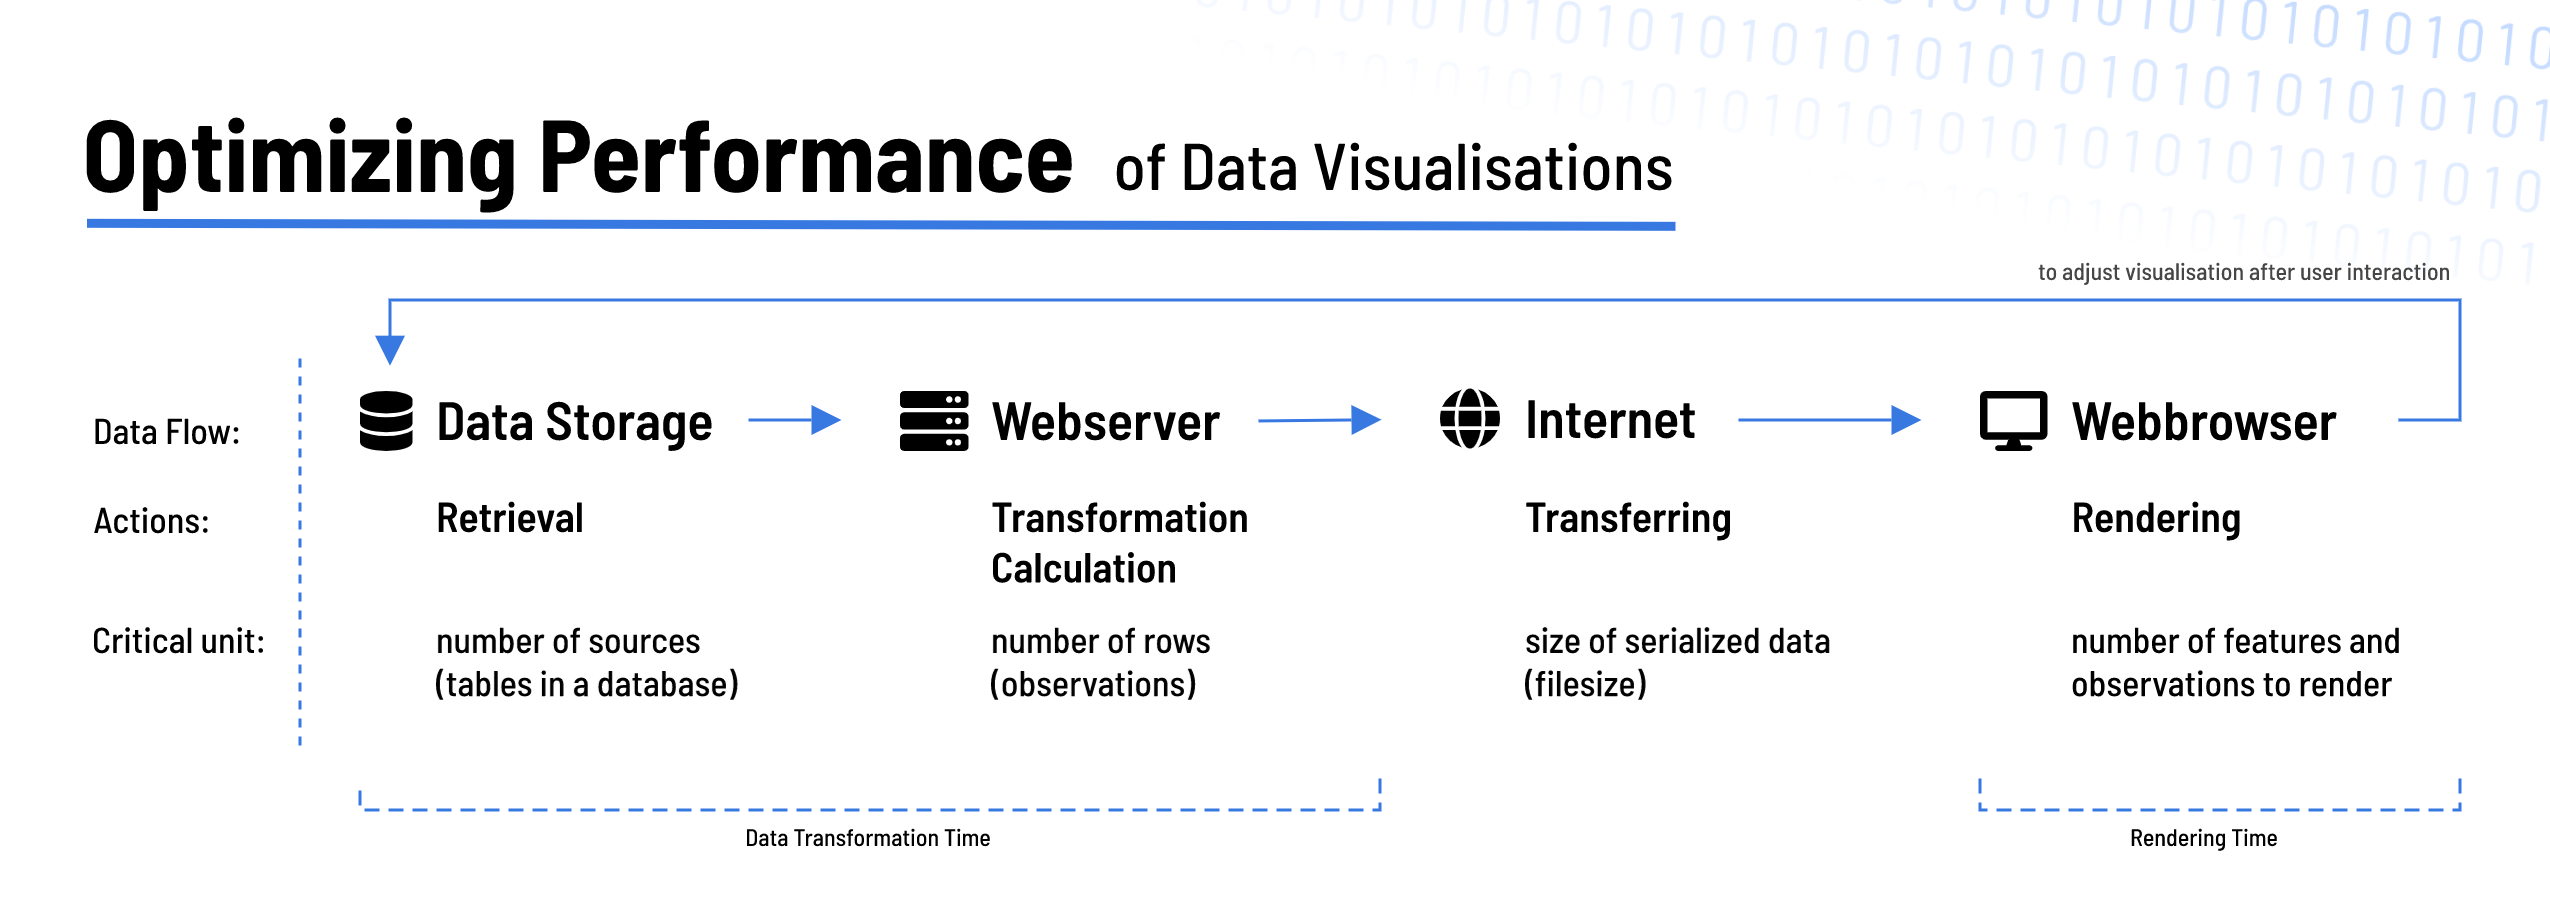
\includegraphics[width=0.7\textwidth]{./performance.png}
    \caption{Infographic showing process to build an interactive visualisation using web technologies. (own graphic)}
\end{figure}

\textit{Figure 1} visualises the four rough parts involved in interactive visualisations built with web technologies. In general, the more data, the more problematic, but the number of sources has a higher impact on data storage systems like databases than the number of features and rows. For example, to transfer data from the webserver to the web browser, only the filesize and the number of requests sent to the server matter. So it is irrelevant if the data consists of a vast amount of rows or attributes. More features affect the web browser's speed slightly more than the webserver since the browser has to add a separate component to the visualisation for every additional feature. Important to know that many web visualisation tools trigger the whole process after most human interactions with the plots.

\subsection{Measurements}

The performance of a visualisation can be quantified by using one of many possible metrics. It is either possible to measure specific overall timeframes or go a step further and use instrumentation to measure individual code blocks ~\cite{isaacs_state_2014}. In web development, a tool called \textit{Lighthouse}~\cite{google_lighthouse_2021} has become the way to measure the performance of websites. It can also be applied to pages containing interactive visualisations and measures specific times like the number of seconds until the user can interact with the site (\textit{Time to Interactive}) or to the point when the first pixel is drawn on it (\textit{First Contentful Paint}).

\begin{wrapfigure}{R}{0.3\textwidth}
    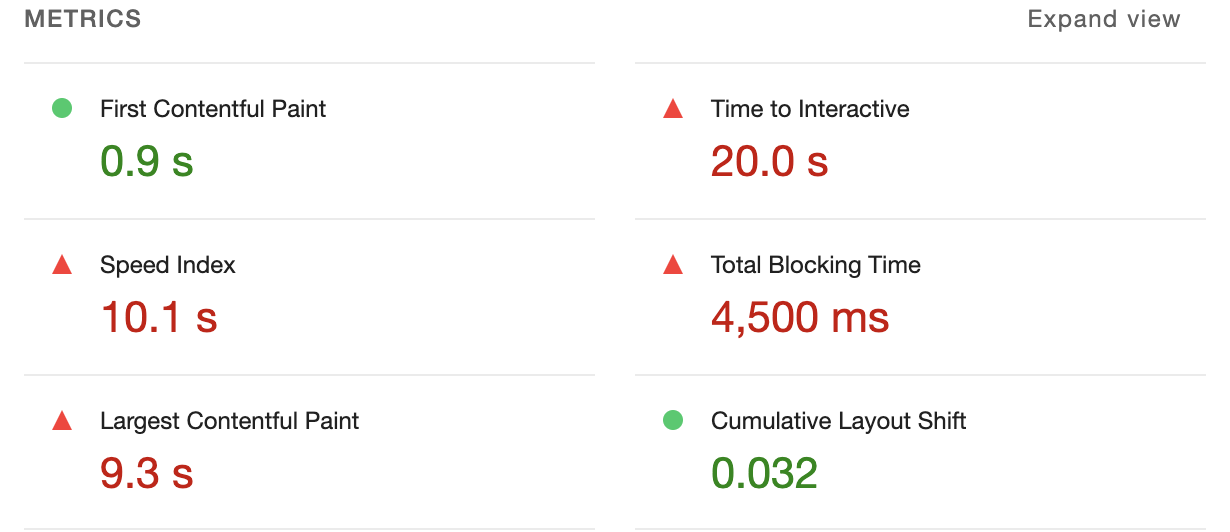
\includegraphics[width=0.3\textwidth]{./lighthouse-1.png}
    \caption{Lighthouse report for dashboard with all observations visible.}
\end{wrapfigure}

The dashboard for the solar energy plant's data suffered severe performance issues. It took quite some time until it got loaded and usable, but each time users changed one of the filters, they had to wait several seconds again for the updated plot. The Lighthouse report (see \textit{Figure 2}) confirms this impression. The total blocking time indicating the cumulated time the user had to wait until the page has been rendered completely is at 4.5 seconds, and the plots have been ready only after 20 seconds. This is too long for a tool to quickly get insights into the data.

\subsection{Solutions}

The possible solutions for slow visualisations are diverse and depend heavily on the problem. If the creation of a plot is deferred because of heavy computations or complex rendering, then outsourcing these tasks to the \textbf{Graphics Processing Unit (GPU)} can speed them up significantly. However, these improvements depend heavily on the available hardware, which is predominantly out of control for data scientists regarding the viewers' machines. For complex visualisations on websites, technologies like \textit{WebGL} should be used, which makes use of the GPU~\cite{mozilla_webgl_2022}.

When showing interactive maps, a technique called \textbf{Tiling} is often used to divide the enormous map into small images to be able to load only the images which are currently in the viewport and required for the current zoom level. This strategy can also be used for other visualisations. For the ones on websites, a library called \textit{Leaflet} is available ~\cite{noauthor_leaflet_2022}.

When calculations after user interactions are not too complex, another improvement is avoiding server roundtrips and recalculating directly in the web browser. However, this is not always possible, primarily when a high-level framework like \textit{Dash} is used. If these can not be bypassed, it is advisable to check for data that can be \textbf{cached}. For example, the ADNI dashboard reloaded the source data on every filter change, which delayed the response by some seconds. However, since the data does not change, it could only be loaded once, and the delay could be removed.

\begin{wrapfigure}{R}{0.3\textwidth}
    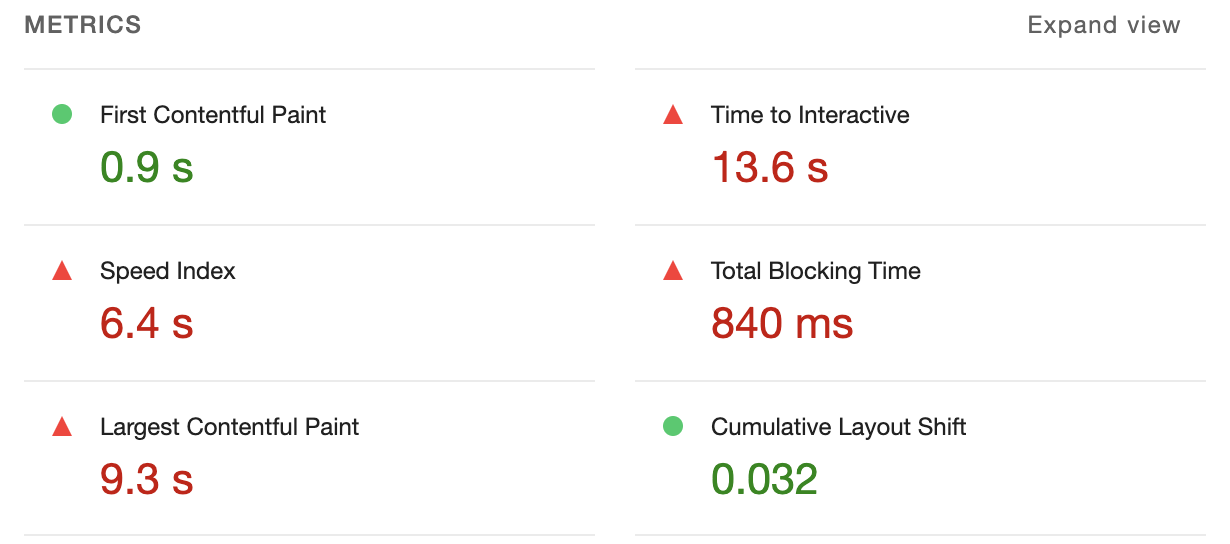
\includegraphics[width=0.3\textwidth]{./lighthouse-2.png}
    \caption{Lighthouse report for dashboard with only observations of one month visible.}
\end{wrapfigure}

Loading data only for one month instead of the complete dataset, which consists of 84'212 observations and 274 attributes, could improve the speed of the energy dashboard. This seemed like a good solution since that much data is overwhelming for the user anyway. Viewers can now switch between months using a filter. Such \textbf{filters} and reducing the \textbf{level of detail} are other practical approaches to improve performance. Certain features could be only shown after the user zoomed into the plot or clicked on specific elements in the plot. If the performance can not be improved anymore and the graphic is still not shown immediately, there should be at least an indicator while the visualisation is rendered. This can be a \textbf{spinner animation} along with a describing text.

\pagebreak
\section{Dashboard Design Principles}
Lorem Ipsum

\pagebreak
\section{HCI Basics}
Lorem Ipsum

\pagebreak
\section{Evaluation}
Lorem Ipsum

\section{Conclusion}
Lorem Ipsum

\pagebreak
\section{Appendix}
Lorem Ipsum

\pagebreak
\bibliographystyle{apacite}
\bibliography{bibliography}


\end{document}